\section{Ablation and Mechanistic Analysis}

\subsection{Same-condition Component Ablations}

Table~\ref{tab:component-evidence} reports the formal component ablations on the occurrence-matched fixed tests. Every comparison uses the same species-specific training and test files, task inventory, three final-training seeds, optimizer, and epoch budget as the locked TissuePMHC model. The no-MHC-branch and no-rank-fusion predictions are derived from the same fitted full models; the no-auxiliary and no-multikernel variants are independently refitted under the same seeds. Task metrics are first averaged across seeds before paired task-wise analysis.

\begin{table*}[t]
\centering
\caption{Formal same-condition ablations on the Human and Mouse occurrence-matched fixed tests. AUROC and AUPRC are task-macro mean $\pm$ sample standard deviation across seeds 20260704--20260706. $\Delta$ AUROC is candidate minus the full model after averaging each task across seeds; brackets give a 10,000-resample task-bootstrap 95\% confidence interval. W/T/L counts tasks with positive/zero/negative deltas. Two-sided paired Wilcoxon $p$-values are Holm-adjusted over the four component contrasts separately within each species. Human has 77 tasks and Mouse has 11.}
\label{tab:component-evidence}
\fontsize{7.2}{8.2}\selectfont
\setlength{\tabcolsep}{2.2pt}
\begin{tabularx}{\textwidth}{@{}llrr>{\raggedleft\arraybackslash}p{3.1cm}rr@{}}
\toprule
Species & System & AUROC & AUPRC & $\Delta$ AUROC [95\% CI] & W/T/L & Holm $p$ \\
\midrule
Human & Full TissuePMHC & $0.8136\pm0.0021$ & $0.8126\pm0.0021$ & --- & --- & --- \\
& No MHC-specific branch & $0.7923\pm0.0017$ & $0.7913\pm0.0014$ & $-0.0213$ [$-0.0265,-0.0164$] & 11/0/66 & $4.45\times10^{-10}$ \\
& No within-task rank fusion & $0.8115\pm0.0027$ & $0.8117\pm0.0022$ & $-0.0021$ [$-0.0036,-0.0007$] & 29/0/48 & 0.0111 \\
& No auxiliary supervision & $0.8169\pm0.0023$ & $0.8156\pm0.0025$ & $+0.0033$ [$-0.0017,+0.0080$] & 45/0/32 & 0.1793 \\
& No multi-kernel encoder & $0.7999\pm0.0037$ & $0.7989\pm0.0036$ & $-0.0137$ [$-0.0189,-0.0084$] & 19/0/58 & $2.13\times10^{-5}$ \\
\midrule
Mouse & Full TissuePMHC & $0.8194\pm0.0157$ & $0.8279\pm0.0121$ & --- & --- & --- \\
& No MHC-specific branch & $0.8133\pm0.0142$ & $0.8218\pm0.0074$ & $-0.0061$ [$-0.0144,+0.0017$] & 4/0/7 & 0.2783 \\
& No within-task rank fusion & $0.8163\pm0.0160$ & $0.8254\pm0.0124$ & $-0.0032$ [$-0.0067,+0.0006$] & 3/0/8 & 0.2031 \\
& No auxiliary supervision & $0.8098\pm0.0147$ & $0.8233\pm0.0141$ & $-0.0096$ [$-0.0155,-0.0035$] & 2/0/9 & 0.0732 \\
& No multi-kernel encoder & $0.7949\pm0.0178$ & $0.8043\pm0.0159$ & $-0.0245$ [$-0.0333,-0.0148$] & 1/0/10 & 0.0117 \\
\bottomrule
\end{tabularx}
\end{table*}

The multi-kernel peptide encoder contributes consistently in both species: replacing it with the position-preserving flattened MLP lowers AUROC by 0.0137 in Human and 0.0245 in Mouse, with confidence intervals excluding zero and Holm-adjusted significance. The MHC-specific branch has a clear Human contribution ($\Delta=-0.0213$); the Mouse estimate has the same direction but is imprecise across only 11 tasks. Within-task rank fusion provides a small Human improvement and a nonsignificant Mouse trend. Auxiliary supervision is species-dependent: its removal does not reduce Human performance, whereas the Mouse point estimate decreases by 0.0096; the latter has unadjusted $p=0.0244$ but does not remain below 0.05 after correction over the four component tests. These are predictive component effects under the fixed benchmark, not evidence that any network branch corresponds to a specific antigen-processing mechanism.

\subsection{Complementarity of Global and Allele-restricted Sharing}

The formal ablation strengthens the earlier architecture-survey observation that global and allele-restricted sharing are complementary. In Human, the global pathway alone (the no-MHC-branch condition) loses 0.0213 AUROC relative to the fitted dual pathway on the same rows and seeds. In Mouse, the corresponding loss is 0.0061 and its task-bootstrap interval crosses zero. Thus, allele-restricted sharing is clearly useful in the larger Human task inventory, while the smaller Mouse benchmark supports only a directionally consistent estimate.

\subsection{Post-hoc Sequence Attribution in Human}

The attribution implementation exactly reproduces all 23,100 saved per-seed Human fixed-test scores (7,700 rows for each of three seeds): the maximum absolute score difference is zero and the Pearson correlation is 1.0000. Across 462 branch--seed--task completeness audits, the median taskwise maximum reconstruction error is 0.0071 logit and the largest is 0.0436. Pairwise seed correlations of residue--position summaries range from 0.8148 to 0.8848, with median Spearman \(r=0.8577\). Thus, the qualitative attribution structure is reproducible across initializations, although this technical stability is not independent biological validation.

Figure~\ref{fig:shap-paired-position} summarizes the paired observed-residue contrast over the 1,540 selected complete fixed-test pairs. The largest descriptive branch-consensus differences occur at P2 (0.6425 logit attribution), P3 (0.4686), and P9 (0.3067). Both fitted branches show the same ordering of these three positions. The P2--P3 concentration indicates that the model places substantial weight on short N-terminal sequence patterns, while the secondary P9 peak is compatible with reliance on a C-terminal anchor position typical of 9-mer MHC-I ligands. This result identifies model-used positions; it does not show that changing one residue would cause tissue-specific presentation.

\begin{figure*}[t]
\centering
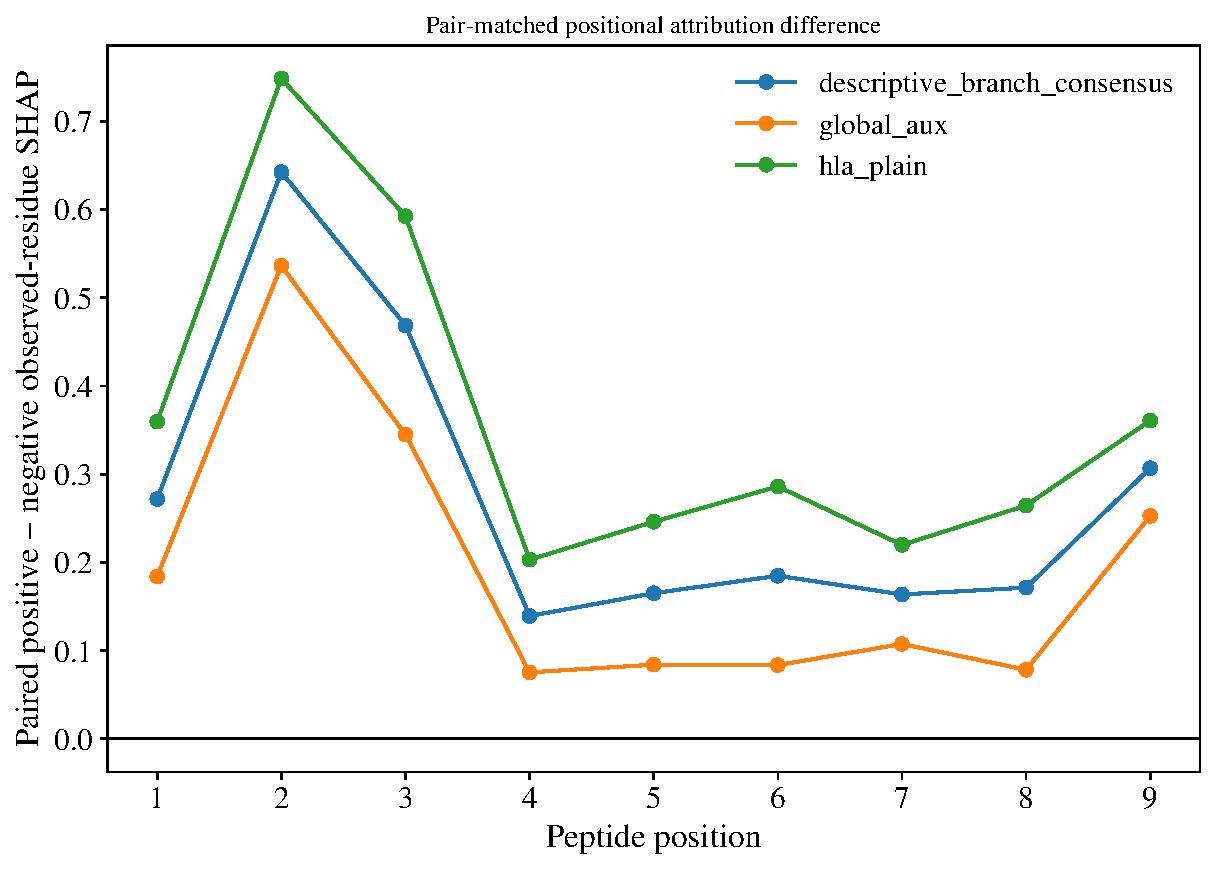
\includegraphics[width=0.86\textwidth]{figures/figure8_shap_paired_position.pdf}
\caption{Pair-matched positional attribution difference for the tuned Human model. For each of 77 tissue--HLA tasks, 20 complete fixed-test pairs are explained under each of three fitted seeds. At each peptide position, the attribution assigned to the recorded-positive peptide's observed residue is subtracted from the corresponding value for its matched pseudo-negative. Curves show the global auxiliary branch, the HLA-specific branch, and their equal-weight descriptive consensus after task- and seed-level aggregation. Values are branch-logit SHAP approximations from task-conditional Expected integrated gradients; the consensus is not an exact decomposition of the non-differentiable percentile-rank fusion.}
\label{fig:shap-paired-position}
\end{figure*}

The HLA-stratified residue maps in Figure~\ref{fig:shap-hla-motifs} further show that positional importance is not explained by one pooled residue pattern. For HLA-A*02:01, for example, L, P, and Y at P2 and V, L, and Y at P9 receive positive contrasts; the HLA-A*24:02 and HLA-B*07:02 panels exhibit different residue--position structures. These maps are more appropriate for motif interpretation than tissue-pooled maps, because pooling by tissue would also mix its observed HLA composition. Nevertheless, each HLA panel still combines tissues, studies, source proteins, and observational sampling. The patterns therefore support an allele-associated sequence interpretation of the fitted model, not discovery of a tissue-specific biochemical mechanism.

\begin{figure*}[t]
\centering
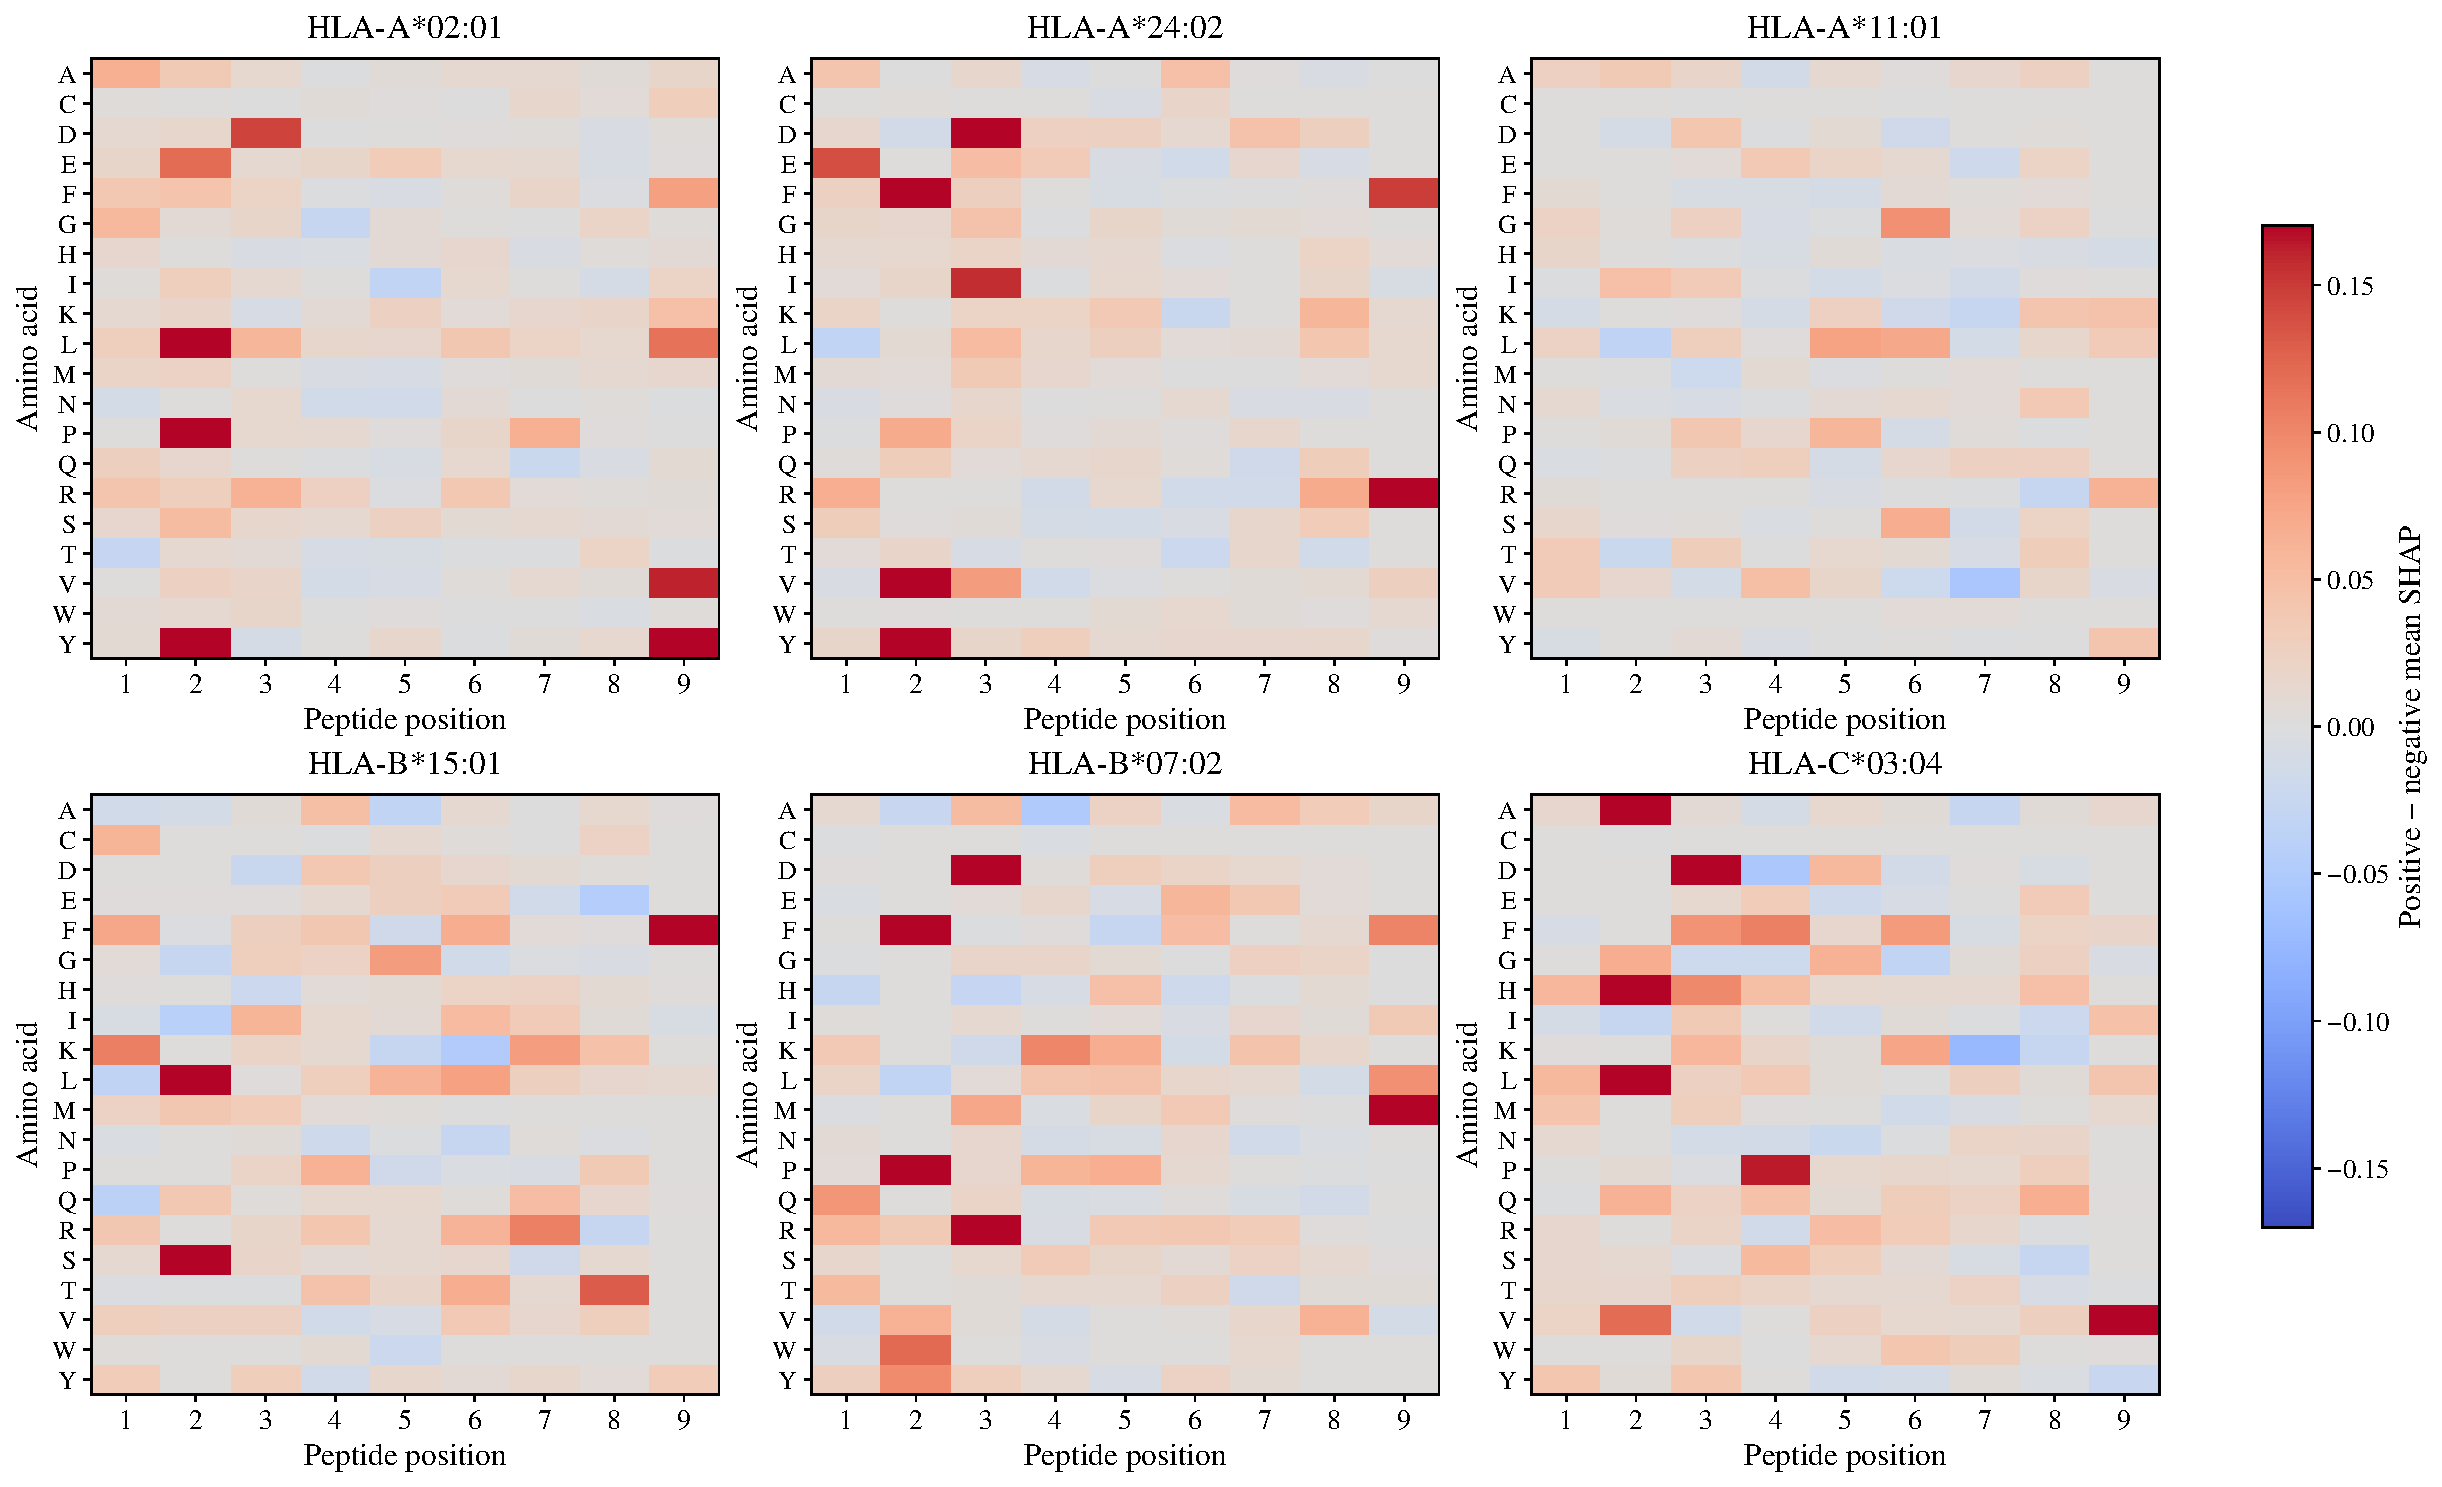
\includegraphics[width=0.98\textwidth]{figures/figure9_hla_shap_motifs.pdf}
\caption{HLA-stratified residue--position attribution maps for six well-represented Human alleles. Each cell is the mean branch-consensus attribution among recorded-positive rows minus that among occurrence-matched pseudo-negative rows for one amino acid and peptide position, aggregated across the three final-training seeds and the represented tissue--HLA tasks. Red indicates that the fitted branches associate that residue--position cell more strongly with the recorded-positive label; blue indicates the reverse. Blank-looking neutral cells are near zero, not missing measurements. Shared color limits permit visual comparison across panels. The maps describe model dependence conditional on task-specific empirical backgrounds and do not establish causal binding or antigen-processing effects.}
\label{fig:shap-hla-motifs}
\end{figure*}

\subsection{Single-residue Perturbation Validation}

SHAP assigns contribution relative to a task-conditional background but does not by itself show how the fitted model responds when a residue is changed. We therefore scored every one of the 526,680 single-amino-acid substitutions defined on the same explained test rows. Reloaded-checkpoint probabilities reproduce the saved branch predictions with maximum absolute error \(4.42\times10^{-7}\), and reconstruction of the original percentile-rank fusion has maximum absolute error \(1.11\times10^{-16}\).

Figure~\ref{fig:ism-validation}a shows the three-seed mean absolute change in the final replacement rank-fusion score. P2 is the most sensitive position (0.1759), followed by P3 (0.1066) and P9 (0.1056); P2 is highest under every seed, while P3 and P9 exchange second and third place. This ordering independently recovers the three positions highlighted by the pair-matched SHAP analysis. For recorded-positive peptides, the mean classification-support losses are likewise largest at P2 (0.0845), P3 (0.0402), and P9 (0.0374). In the prespecified within-peptide comparison, mean P2/P9 sensitivity exceeds the other seven positions by 0.0590 (2,000-resample 95\% CI 0.0566--0.0615; one-sided Wilcoxon Benjamini--Hochberg \(q<10^{-300}\)). This pooled anchor comparison supports the position-level result but does not imply that every represented HLA uses identical anchor chemistry.

The direct sample--position comparison in Figure~\ref{fig:ism-validation}b--c also links the two explanation families. After averaging each quantity across the three fitted seeds, observed-residue Expected-IG attribution correlates with mean ISM mutation loss at Spearman \(\rho=0.827\) for the global auxiliary branch and \(\rho=0.911\) for the HLA-specific branch. The corresponding per-seed correlations have medians 0.787 and 0.882. Thus, residues assigned a positive contribution relative to the empirical background generally lose branch logit when replaced, providing an independent perturbation check on the attribution direction.

The validation is stronger at the position level than at the exact substitution level. Across the 3,420 position--original-residue--mutant-residue cells, pairwise seed correlations for final rank-fusion effects range from 0.527 to 0.587 (median 0.541), despite the stable P2/P3/P9 ordering. We therefore interpret ISM as support for the positional attribution pattern, not as a seed-invariant catalogue of beneficial or deleterious amino-acid substitutions.

\begin{figure*}[t]
\centering
\makebox[\textwidth][c]{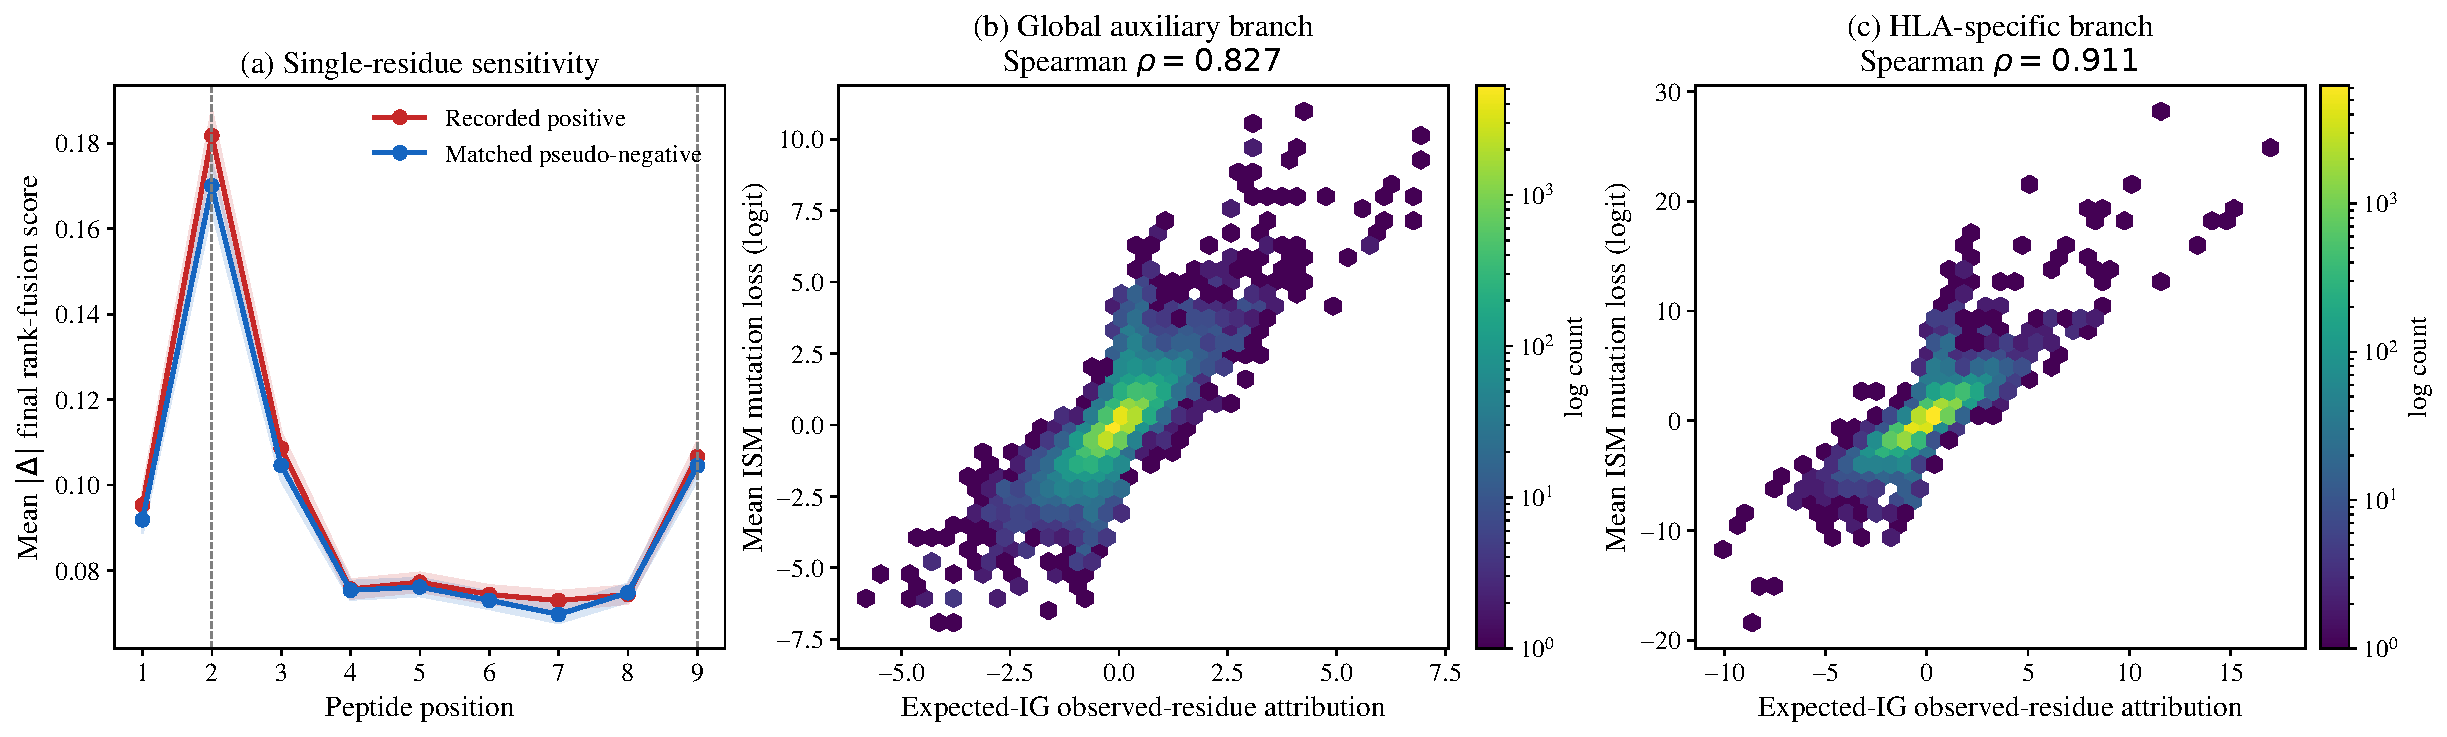
\includegraphics[width=1.10\textwidth]{figures/figure10_ism_validation.pdf}}
\caption{Exhaustive single-residue in silico mutagenesis (ISM) validation of the Human attribution result. (a) For each selected peptide and position, sensitivity is the mean absolute change in the final within-task replacement rank-fusion score over the 19 alternative amino acids; curves show the three-seed mean for recorded-positive and matched pseudo-negative rows, with 95\% normal intervals over peptides. Dashed lines mark P2 and P9. (b--c) Hexagonal-bin comparisons between the observed-residue Expected-IG attribution and the mean ISM branch-logit loss over the 19 substitutions, after averaging both quantities across the three fitted seeds. Correlations use all 27,720 sample--position observations per branch. ISM measures fitted-model response to computational substitutions and does not establish an in vivo mutation effect.}
\label{fig:ism-validation}
\end{figure*}

The same-HLA counterfactual analysis tests whether this response changes when only the tissue task is switched. Across the 28 HLA alleles represented in multiple tissues, the equal-HLA mean absolute difference between tissue-task rank-fusion effects is 0.1703, compared with 0.0871 across training seeds within a task. The median HLA-level tissue-to-seed dispersion ratio is 1.899 (range 1.404--2.754); tissue dispersion exceeds seed dispersion for all 28 HLA alleles, and all peptide-level paired tests remain significant after correction (one-sided Wilcoxon, Benjamini--Hochberg \(q<0.05\)). Across the 96 same-HLA tissue-task pairs, mutation-effect rankings have median Spearman \(\rho=-0.266\) and median sign disagreement 0.596, indicating that the task change often alters more than effect magnitude. Tissue-contrast vectors have moderate cross-seed reproducibility (median Spearman \(\rho=0.608\)), so exact task-specific substitutions remain less stable than the pooled position ordering.

Figure~\ref{fig:cross-tissue-ism} makes this task dependence easier to read at two scales. In the HLA-level lollipop display, all 28 estimates have positive $\log_2$(tissue/seed) ratios and peptide-bootstrap 95\% intervals above zero. The HLA-A*02:01 fingerprint then shows which tissue tasks depart above or below that allele's cross-tissue positional baseline; P2, P3 and P9 are highlighted because they have the largest pooled tissue dispersion (0.3074, 0.1920 and 0.1798, respectively). Thus, the P2/P3/P9 pattern is shared at the pooled level, but the direction and magnitude of a fixed substitution are substantially modulated by the fitted tissue task even when HLA and peptide are held constant. This is direct evidence of model-level tissue conditioning, not evidence that a particular tissue process causes the contrast.

\begin{figure*}[t]
\centering
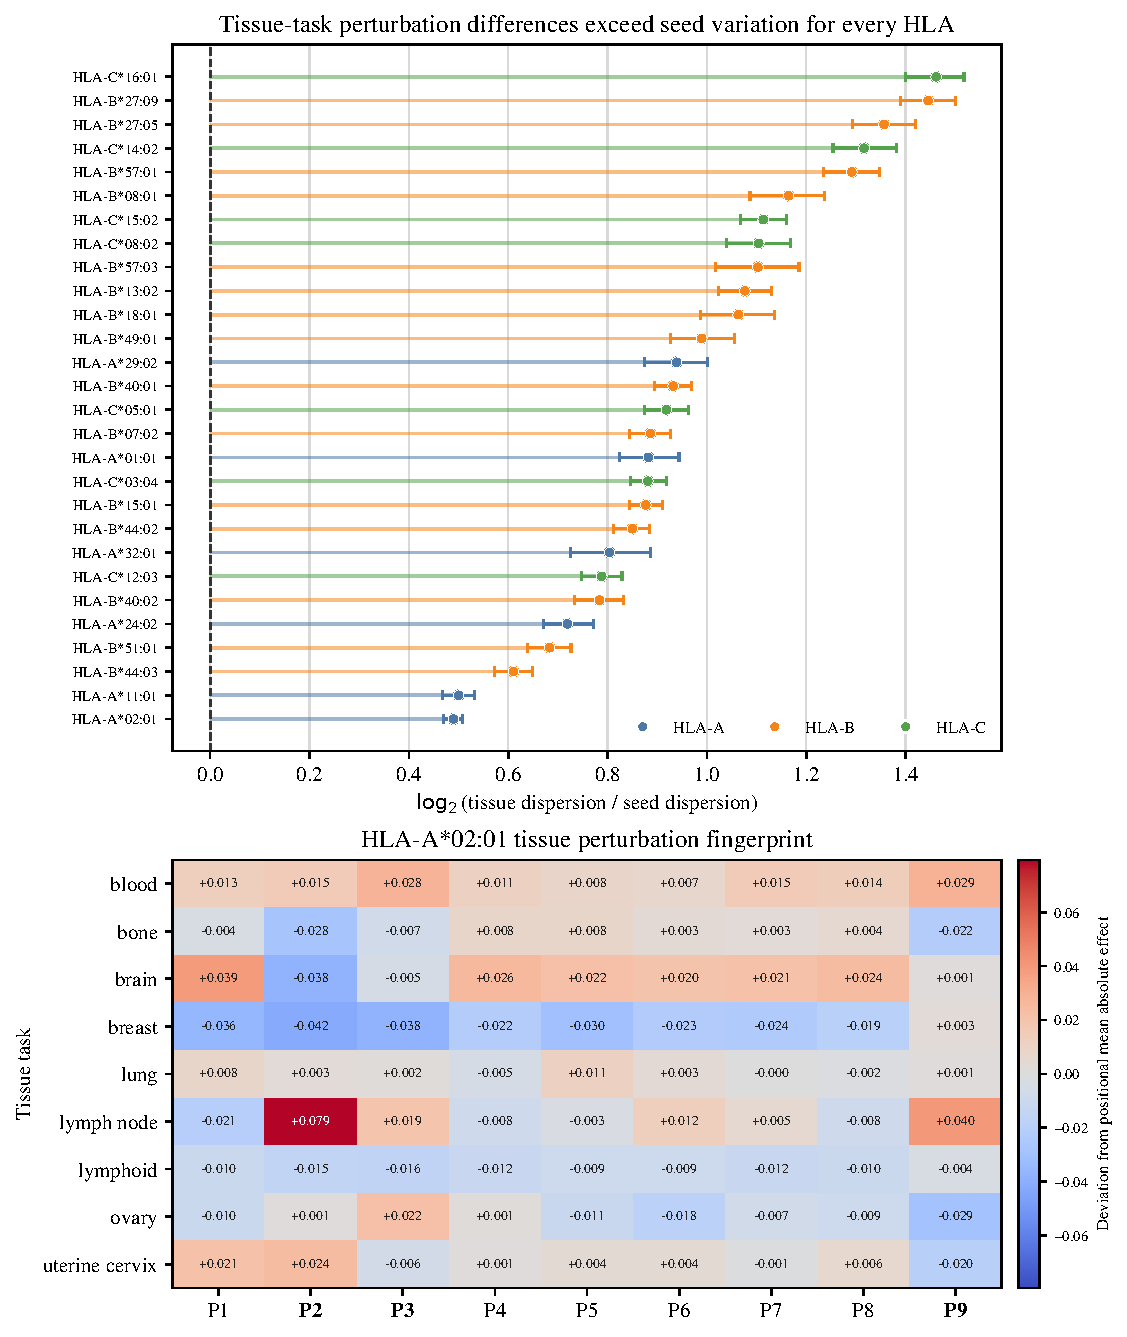
\includegraphics[width=\textwidth]{figures/figure11_cross_tissue_ism.pdf}
\caption{Counterfactual same-HLA comparison of single-residue perturbation effects across Human tissue tasks. Each fixed peptide, position and substitution is scored under every represented tissue task for the same HLA. (a) HLA-level $\log_2$(tissue/seed) dispersion ratios for the final rank-fusion perturbation effect: dots are point estimates, horizontal bars are peptide-bootstrap 95\% intervals and colour denotes HLA locus; the dashed line marks equal tissue and seed dispersion. (b) A representative HLA-A*02:01 tissue perturbation fingerprint. Each cell is the three-seed mean absolute rank-fusion effect at one peptide position in one annotated tissue task, centred by the allele's across-tissue mean for that position. Red and blue denote above- and below-baseline sensitivity; P2, P3 and P9 are emphasized. These contrasts establish fitted-model task dependence under fixed peptide and HLA inputs; they do not identify a causal tissue-processing mechanism.}
\label{fig:cross-tissue-ism}
\end{figure*}
